\documentclass{article}
\usepackage{amsmath, amsthm, amssymb, amsfonts}
\usepackage{thmtools}
\usepackage{graphicx}
\usepackage{setspace}
\usepackage{geometry}
\usepackage{float}
\usepackage{hyperref}
\usepackage[utf8]{inputenc}
\usepackage[english]{babel}
\usepackage{framed}
\usepackage[dvipsnames]{xcolor}
\usepackage{tcolorbox}
\usepackage{ dsfont }
\usepackage{ mathtools }
\usepackage{ tipa }

\colorlet{LightGray}{White!90!Periwinkle}
\colorlet{LightOrange}{Orange!15}
\colorlet{LightGreen}{Green!15}

\graphicspath{ {./pictures/} }

\newcommand{\HRule}[1]{\rule{\linewidth}{#1}}

% ------------------------------------------------------------------------------

\begin{document}

% ------------------------------------------------------------------------------
% Cover Page and ToC
% ------------------------------------------------------------------------------

\title{ \normalsize \textsc{}
		\\ [2.0cm]
		\HRule{1.5pt} \\
		\LARGE \textbf{\uppercase{ Mathe Hausübung Nr. 4 }
        \HRule{2.0pt} \\ [0.6cm] \LARGE{ Sebastian Steitz, Hannes Albert } \vspace*{10\baselineskip}}
		}
\date{Mai 2023}
\author{\textbf{} \\
		Gruppe: 6 \\
		Tutor: Zidane Bührmann }

\maketitle

\setlength\leftskip{1cm}
\section{4.1}
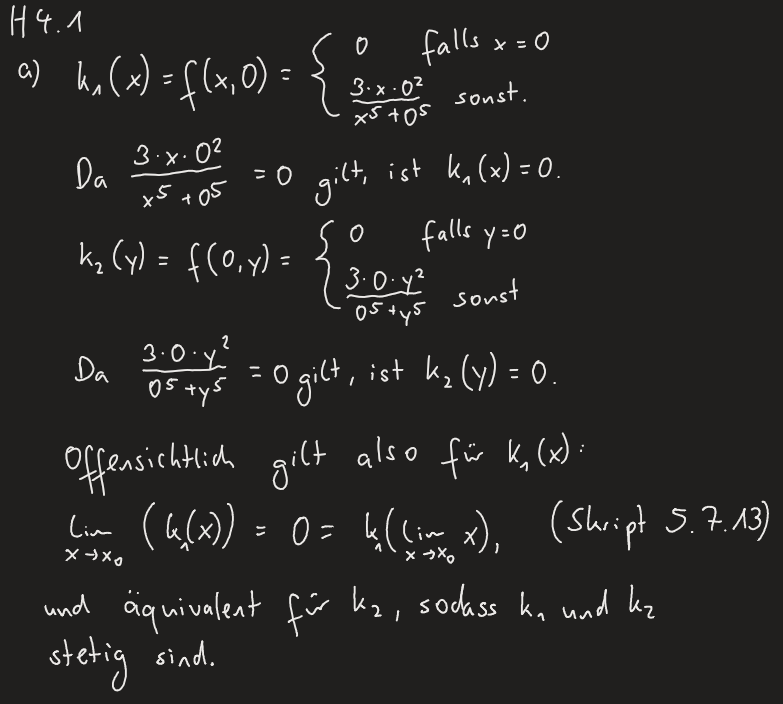
\includegraphics[scale=0.7]{ h4_1a } \\ 
\bigskip

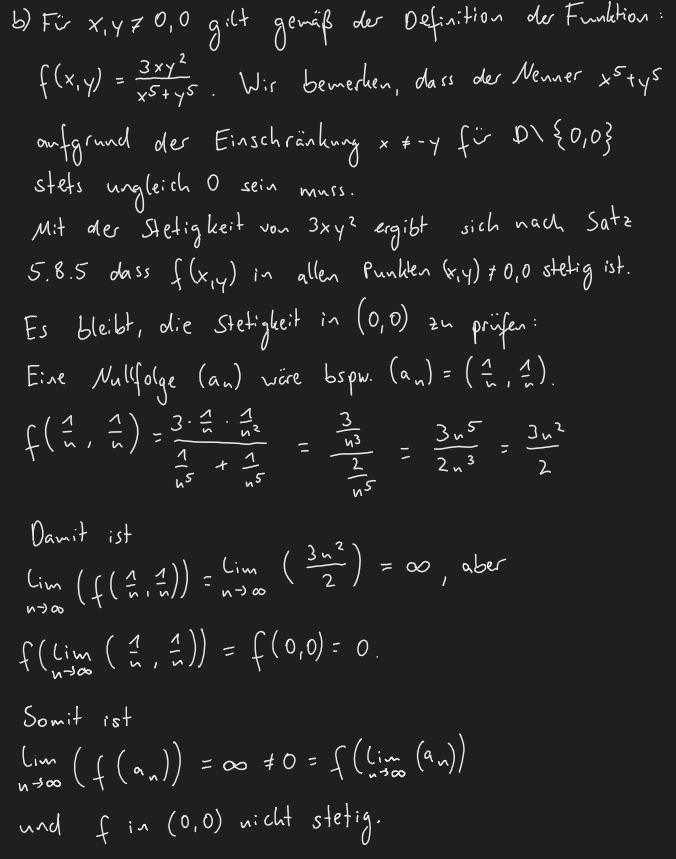
\includegraphics[scale=0.7]{ h4_1b } 
\newpage

\section{H4.2}
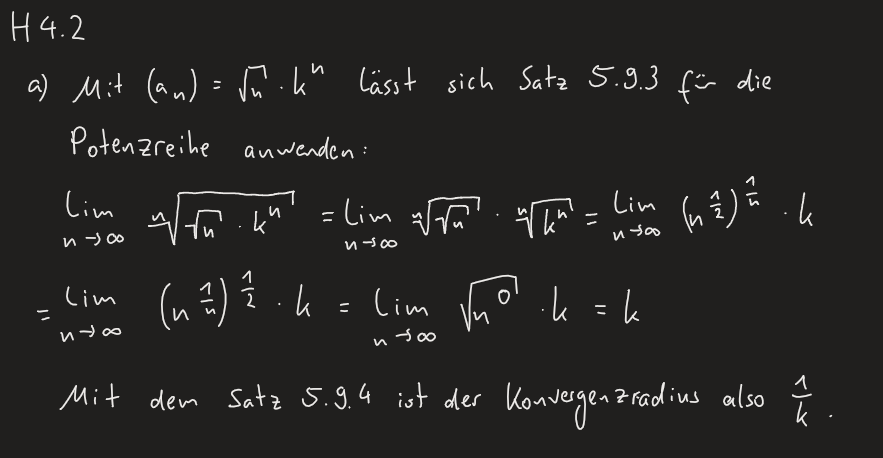
\includegraphics[scale=0.6]{ h4_2a }
\bigskip

\noindent b) \\ 
Zunächst untersuchen wir die Potenzreihe, gemäß Satz 5.9.3, auf einen möglichen Grenzwert $\varrho$.
Hierfür lesen wir die Folge $(a_n)_{n \in \mathds{N}}$ := $n^2$ * $3^n$ ab. Damit gilt:
\begin{align*}
    \varrho & = \lim_{n \to \infty} \sqrt[n]{\left| a_n \right|} = \lim_{n \to \infty} \sqrt[n]{\left| n^2 * 3^n \right|}
    \overset{n^2 \geq 0 \text{ } 3^n \geq 0}{=} \lim_{n \to \infty} \sqrt[n]{n^2 * 3^n} \\
    & = \lim_{n \to \infty} \sqrt[n]{n^2} * \sqrt[n]{3^n} 
    = \lim_{n \to \infty} \sqrt[n]{n^2} * 3  
    = 3 * \lim_{n \to \infty} \sqrt[n]{n^2} \\  
    & = 3 * \lim_{n \to \infty} \sqrt[n]{n} * \sqrt[n]{n}  
    = 3 * \lim_{n \to \infty} (n^{\frac{1}{n}} * n^{\frac{1}{n}}) \\ 
    & = 3 
\end{align*}
Da 3 $\in$ (0, $\infty$) gilt hier Fall (c) von Satz 5.9.3
Mithilfe von Satz 5.9.3 lassen sich somit auch Aussagen über das Konvergenzverhalten der Potenzreihe treffen. So
gilt für alle x $\in \mathds{R}$ mit $\left| x - 1 \right|$ $<$ $\frac{1}{3}$ konvergiert und für alle 
x $\in \mathds{R}$ mit $\left| x - 1 \right|$ $>$ $\frac{1}{3}$ divergiert. \\
Wir betrachten: 
\begin{align*}
    \left| x - 1 \right| & = \frac{1}{3} \\
    \overset{+}{-}(x - 1) & = \frac{1}{3} \\
    \medskip
    1.Fall \\
    x_1 - 1 & = \frac{1}{3} \\ 
    x_1 & = \frac{4}{3} \\ 
    \medskip
    2.Fall \\
    -(x_2 - 1) & = \frac{1}{3} \\ 
    -x_2 + 1 & = \frac{1}{3} \\ 
    -x_2 & = -\frac{2}{3} \\ 
    x_2 & = \frac{2}{3}
\end{align*}
Dies bedeuted, dass die Potenzreihe für alle x $\in$ ($\frac{1}{3}$, $\frac{2}{3}$) konvergiert. Da wir wissen,
dass 
\[
    \forall x \in [\frac{1}{3}, \frac{2}{3}] :\text{ } \left| x - 1 \right| \leq \frac{1}{3} 
\]
Daraus lässt sich schließen, dass für alle x $\in$ $\mathds{R}$ $\backslash$ [$\frac{1}{3}$, $\frac{2}{3}$] die Potenzreihe divergiert.
Damit müssen wir nur noch die Randfälle, also x = $\frac{1}{3}$ und x = $\frac{2}{3}$ betrachten. \\
\smallskip
x = $\frac{1}{3}$: 
\begin{align*}
    n^2 * 3^n * (\frac{1}{3} - 1)^n & = n^2 * 3^n * (- \frac{2}{3})^n \\ 
                                    & = n^2 * (-2)^n
\end{align*}
Da es sich hiermit um keine Nullfolge handelt folgt aus Satz 5.5.5, dass es sich für x = $\frac{1}{3}$ und eine divergente Reihe handelt. \\
\smallskip
x = $\frac{2}{3}$:
\begin{align*}
    n^2 * 3^n * (\frac{2}{3} - 1)^n & = n^2 * 3^n * (- \frac{1}{3}) \\ 
                                & = n^2 * (-1)^n
\end{align*}
Hier handelt es sich auch um keien Nullfolge weswegen die Reihe für x = $\frac{2}{3}$ aus den selben Gründen divergiert, 
wie für x = $\frac{1}{3}$.

\newpage
\section{H4.3}
\noindent a) \\ 
\bigskip

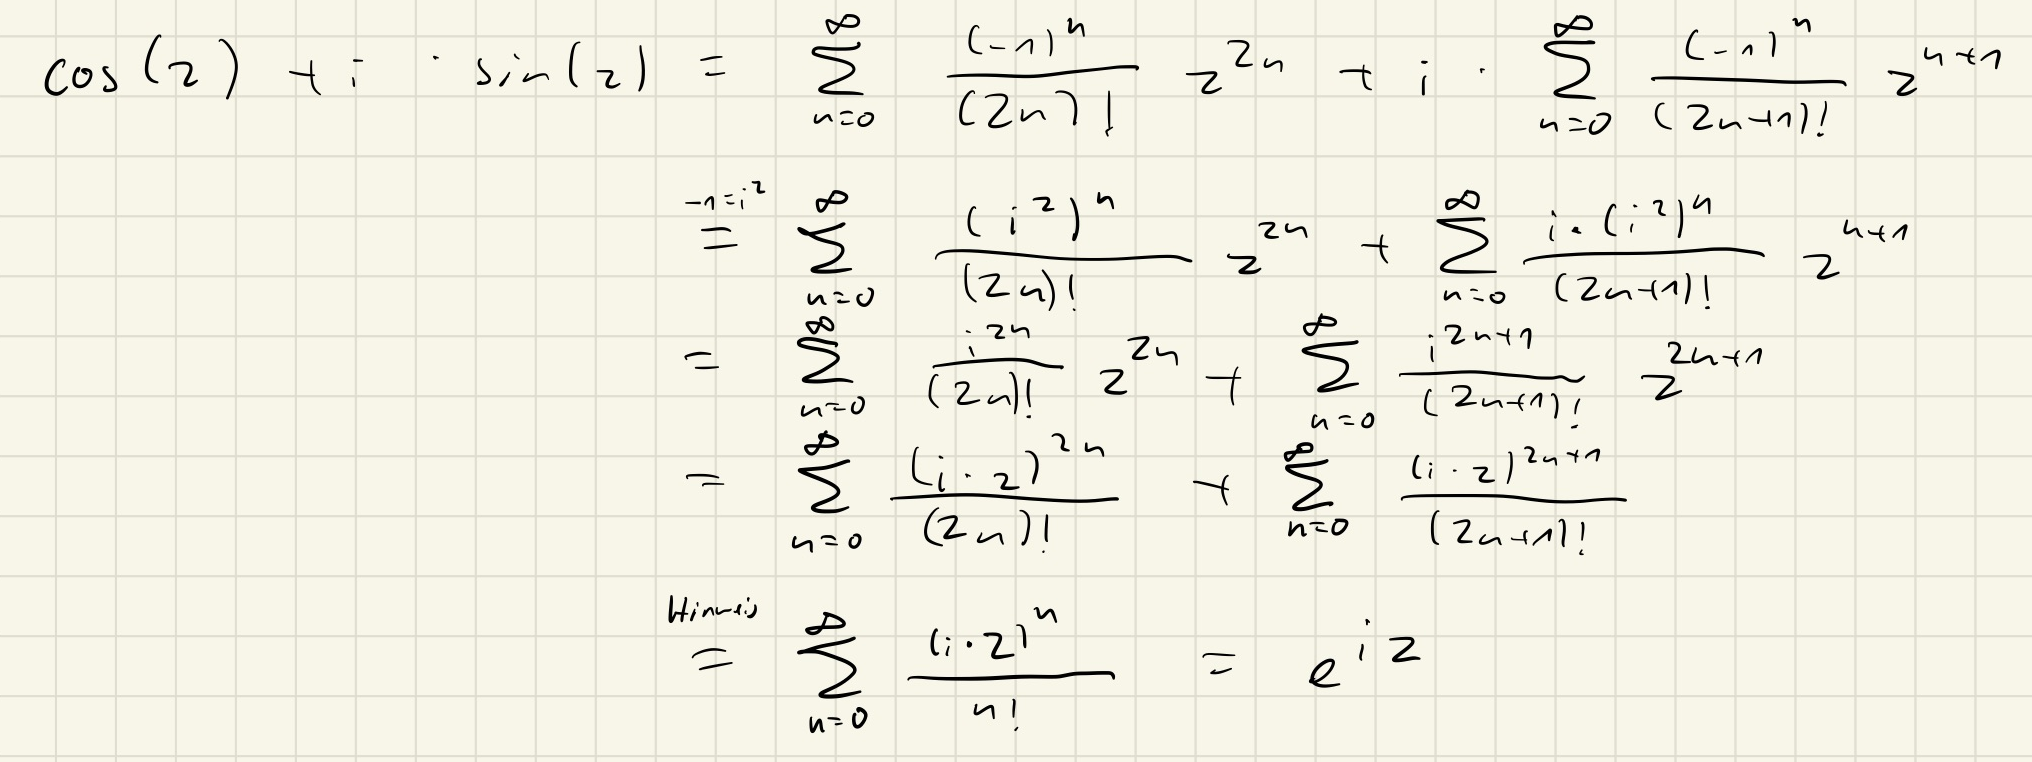
\includegraphics[scale=0.225]{ h4_3a } \\ 
Wir dürfen den Hinweis hier verwenden, da in Beispiel 5.5.18 bereits die absolute Konvergenz von e gezeigt wurde.

\bigskip
\noindent b) \\ 
Für den Cosinus gilt folgendes: 
\begin{align*}
    cos(z) & = \frac{e^{iz} - e^{-iz}}{2} \\
           & = \frac{cos(z) + i * sind(z) + cos(z) - i * sin(z)}{2} \\ 
           & = \frac{2 * cos(z)}{2} \\ 
           & = cos(z)
\end{align*}
\smallskip
Und für den Sinus folgendes:
\begin{align*}
    sin(z) & = \frac{cos(z) + i * sin(z) - (cos(z) - i * sin(z))}{2 * i} \\ 
           & = \frac{cos(z) + i * sin(z) - cos(z) + i * sin(z)}{2 * i} \\ 
           & = \frac{i * sin(z) + i * sin(z)}{2 * i} \\ 
           & = \frac{2 * i * sin(z)}{2 * i} \\ 
           & = sin(z)
\end{align*}
\end{document}

